\chapter{Lecture 27 - Sub-cooled Nucleate Boiling}
\label{ch:ch27}
\section{Objectives}
The objectives of this lecture are:
\begin{enumerate}
\item Describe bulk coolant properties in a PWR fuel assembly in the context of two-phase flow.
\item Describe correlations to predict the onset of sub-cooled nucleate boiling and convective heat transfer coefficients for sub-cooled nucleate boiling.
\item Show an example calculation (in MATLAB) for an AP1000.
\end{enumerate}

\section{Heat Flux and Temperature in a PWR Fuel Channel}
\begin{marginfigure}
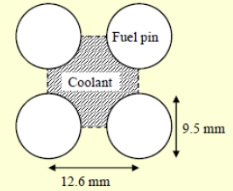
\includegraphics[width=2.5cm]{single_channel.png}
\caption{Representative channel in a PWR.}
\label{fig:single_channel}
\end{marginfigure}
To simplify the discussion, we will consider a representative fuel channel in a PWR similar to what is depicted in Figure \ref{fig:single_channel}.  If, for the time being, we simplify further by assuming that the power generated within the pin, and thus the heat flux at the pin boundary, is constant.  We might expect a flow and temperature profile like what is depicted in Figure \ref{fig:channel-temp-and-heat-flux}.

\begin{marginfigure}
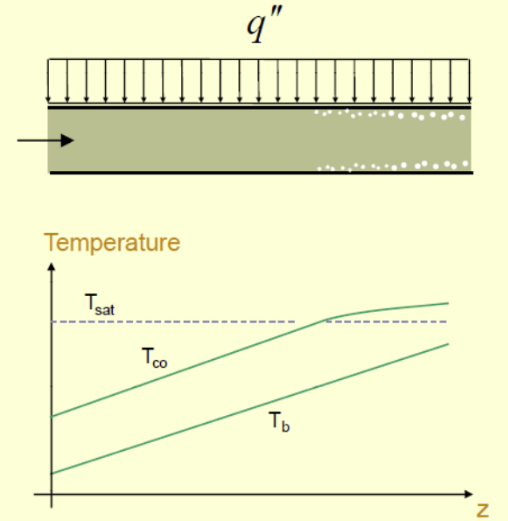
\includegraphics{channel-temp-and-heat-flux.png}
\caption{Temperature and heat flux profile for simplified channel.}
\label{fig:channel-temp-and-heat-flux}
\end{marginfigure}

\newthought{Some observations} you might make about this flow configuration:
\begin{itemize}
\item Sub cooled liquid is assumed to enter the the channel and heat transfer initially is via sub cooled forced convection.
\item In the sub cooled forced convection region, the $\Delta T$ between the coolant and the cladding outer surface $T_{co} - T_b$ is roughly constant since the heat flux and linear heat rate are constant.
\item The temperature of the coolant increases due to the accumulated energy transferred from the fuel pin to the coolant, so both $T_{b}$ and $T_{co}$ increase more-or-less linearly.
\item When $T_{co}$ gets above $T_{\text{sat}}$, voids begin to form along the fuel clad outer surface.  The process of this bubble formation will be discussed in the next section, but bubbles formed at \emph{nucleation sites} result in enhanced convective heat transfer between the clad surface and the bulk coolant.  When this occurs, $\Delta T$ between the clad and coolant starts to decrease.
\item As sub cooled nucleate boiling gets more intense, the heat transfer between the clad and coolant continues to improve and the $\Delta T$ continues to get smaller.  This explains the shape at the right-end of Figure \ref{fig:channel-temp-and-heat-flux}.
\end{itemize}

%\begin{marginfigure}
%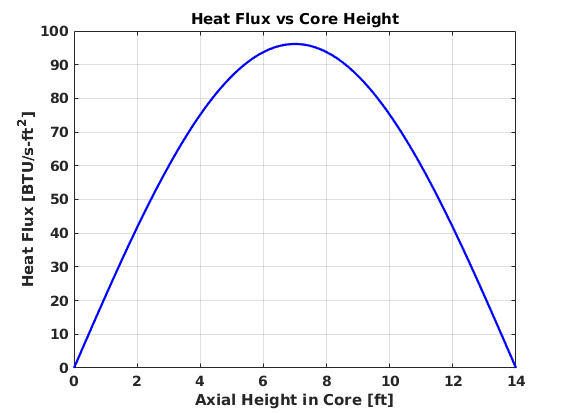
\includegraphics{heat-flux-vs-height.png}
%\caption{A Cosine-shaped heat flux profile.}
%\label{fig:heat-flux-vs-height}
%\end{marginfigure}
\begin{marginfigure}
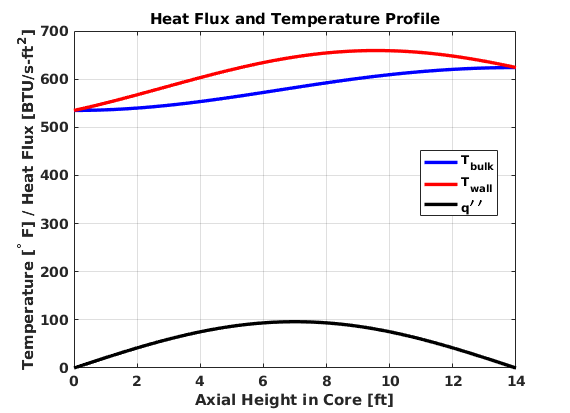
\includegraphics{temperature-and-heat-flux-cosine.png}
\caption{Temperature in a channel with cosine flux distribution using Presser correlation.}
\label{fig:temperature-and-heat-flux-cosine}
\end{marginfigure}
\newthought{Of course} a realistic heat flux profile would not be flat.  A better approximation would be to use a cosine-shaped flux profile.  If we assume this heat flux, we can, using tools already presented, estimate bulk coolant and wall temperature using the Presser correlation for convective heat transfer coefficient in a typical AP1000 fuel assembly.  This is presented in Figure \ref{fig:temperature-and-heat-flux-cosine}.\marginnote{\textbf{Note:} see how the maximum clad temperature $(T_{\text{wall}})$ is reached in the upper half of, but not the top of, the core.}

\section{Sub-cooled Nucleate Boiling}
A phenomena that we have not taken into account is the possibility of sub-cooled nucleate boiling.  For the heat flux profile and convective heat transfer correlations that we have been using, the wall temperature eventually exceeds saturation temperature for the nominal pressure.\sidenote[][-1.0cm]{Please note that this demonstration has not taken into account axial variation in local pressure due to hydrostatic effects or due to major or minor head losses.} If we superimpose the nominal saturation temperature on a plot of $T_{\text{wall}}$ we get the result shown in Figure \ref{fig:wall-temp-and-saturation-temp}.
\begin{marginfigure}
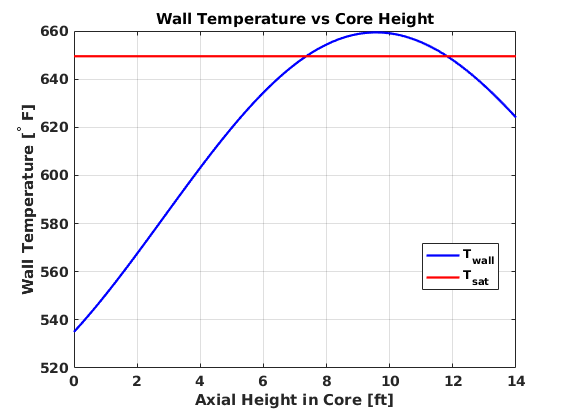
\includegraphics{wall-temp-and-saturation-temp.png}
\caption{Wall temperature compared to saturation temperature in an AP1000 channel.}
\label{fig:wall-temp-and-saturation-temp}
\end{marginfigure}
A schematic of the process of sub-cooled nucleate boiling is shown in Figure \ref{fig:nucleation-schematic}.  When wall temperature exceeds saturation temperature, local voids of saturated vapor can form at nucleation sites, which are small pores, cracks or scratches in the clad surface.  Since the wall temperature exceeds saturation temperature, the pressure of the vapor in the bubble exceeds nominal static pressure; that super-heat is needed so the internal bubble pressure can overcome static pressure plus the surface tension of the bubble.  As wall temperature increases locally, the vapor bubble can grow.  Ultimately the vapor bubble is drawn away from the wall, at least in part, due to forces exerted by the sub-cooled liquid flowing along the surface.
\begin{marginfigure}
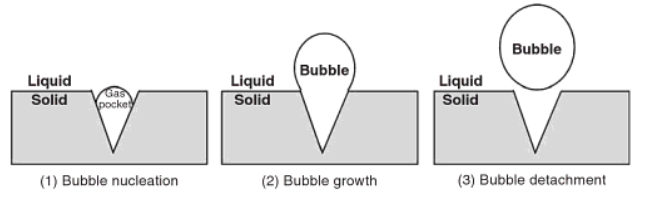
\includegraphics{nucleation-schematic.png}
\caption{Schematic of the sub-cooled nucleation process.}
\label{fig:nucleation-schematic}
\end{marginfigure}

\section{Correlations to Predict Onset of Sub-cooled Nucleate Boiling}
We will present two correlations to predict the onset of nucleate boiling.  The Jens-Lottes correlation is given in USCS units in Equation \ref{eq:jens-lottes-uscs}. \index{Jens-Lottes correlation}
\begin{equation}
T_{\text{wall,ONB}}(z) = T_{\text{sat}}+1.897e^{-\sfrac{P}{900}}\left(q^{\prime \prime}(z) \right)^{0.25}
\label{eq:jens-lottes-uscs}
\end{equation}
where $T_{\text{wall,ONB}}$ and $T_{\text{sat}}$ are in $^{\circ}$F, $P$ is in psia, $500 < P < 2250$, $q^{\prime \prime}$ is in BTU/hr-ft$^{2}$, and $z$ is axial position in feet.

Jens-Lottes in SI units is: 
\begin{equation}
T_{\text{wall,ONB}}(z) = T_{\text{sat}}+45e^{-\sfrac{P}{62}}\left(q^{\prime \prime}(z) \right)^{0.25}
\label{eq:jens-lottes-si}
\end{equation}
where $T$ is in C$^{\circ}$, $P$ is in bar, $q^{\prime \prime}$ is in MW/m$^{2}$, and $z$ is axial position in meters.

The Thom correlation can also be used. In USCS units it is as shown in Equation \ref{eq:thom-uscs}.
\begin{equation}
T_{\text{wall,ONB}}(z) = T_{\text{sat}}+0.072e^{-\sfrac{P}{630}}\left(q^{\prime \prime}(z) \right)^{0.25}
\label{eq:thom-uscs}
\end{equation}

\newthought{Using both} the Thom and Jens-Lottes correlation for this example, the predicted temperature for onset of nucleate boiling is shown in Figure \ref{fig:onb-prediction-ap1000}.  Where the wall temperature is greater than $T_{\text{wall,ONB}}$, we predict nucleate boiling to take place.
\begin{marginfigure}
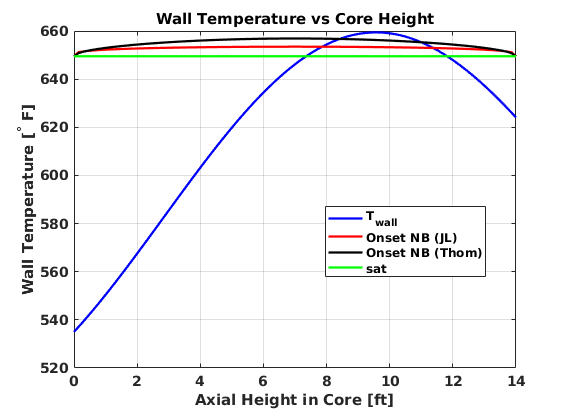
\includegraphics{onb-prediction-ap1000.png}
\caption{Prediction of onset of nucleate boiling using Jens-Lottes and Thom correlation.}
\label{fig:onb-prediction-ap1000}
\end{marginfigure}

\section{Correlation for Sub-cooled Nucleate Boiling}
Where we expect nucleate boiling to take place, we also expect enhanced convective heat transfer.  This effect is not captured in any of the other correlations that we have presented. We will use the Bernath correlation for convective heat transfer in the sub-cooled nucleate boiling regime, which is given by Equation \ref{eq:bernath}.

\begin{equation}
h_{\text{NB}} = 10,890\left(\frac{D_e}{D_e^{\prime}} \right) + \frac{48v}{D_e^{0.6}}
\label{eq:bernath}
\end{equation}
where $D_e$ is the usual hydraulic diameter, $D_e = \sfrac{4 A_{\text{flow}}}{P_{\text{wetted}}}$; $D_e^{\prime} = D_e + \sfrac{P_{\text{heated}}}{\pi}$, and $v$ is average velocity in feet per second.

The complete code for calculations presented in this lecture is provided in the appendix.

\section{Considerations for More Detailed Analysis}
This lecture dealt with a highly simplified thermal model of a typical cooling channel in a PWR fuel assembly.  Some thoughts are presented below as to how this analysis could be improved.

\begin{itemize}
\item \emph{Obtain a more accurate axial power distribution.}  The actual power distribution in a PWR core may not be cosine-shaped but instead will normally be skewed towards the bottom of the core due to coolant temperature/density variation and the feedback that has on core physics and power generation.  For PWRs that use boric acid for reactivity control, boron may be preferentially deposited at sites where nucleate boiling occurs; this can result in the power distribution to be further shifted towards the lower portions of the core.  These changes will impact the core height at which nucleate boiling can be expected to occur; they may also result in higher-than-expected fuel and clad temperatures than would otherwise occur.

\item \emph{Account for variation in cooling channel inlet pressure and velocity.}  For typical PWRs operating today, the flow-path required for water coming in from the cold leg results in wide variation in the inlet pressure and velocity for cooling channels.  This can result in some channels having lower inlet pressure and lower inlet mass flow rate than some other channels.  While much of this effect is mitigated by mixing between adjacent channels it reduces the accuracy of simplified analysis of this sort.

\item \emph{A better analysis would take into account the variation of pressure between channel inlet and outlet.}  For vertically oriented reactor cores, static pressure is reduced near the core outlet due to hydrostatic pressure variation.  No matter how the core is oriented, major and minor head losses will result in a reduction in static pressure as the coolant flows through the core.  Both of these effects would result in lower saturation temperature; nucleate boiling as well as other two-phase flow phenomena would begin lower in the core than this analysis would predict and overall the core would be closer to thermal limits than this analysis assumes.

\item \emph{Account for hydraulic and thermal communication between channels.} In a real LWR core, coolant mixes between adjacent channels carrying thermal and flow energy with it.  

\item \emph{Use more correlations.}  In this lecture I have presented only a subset of all available correlations for convective heat transfer and onset of nucleate boiling.  For a novel reactor design it is almost sure to be the case that extensive experiments will need to be done to evaluate actual core thermal performance under safe conditions.

Modern computer codes used in the nuclear industry capture all of these considerations and more.  Sadly, their theory and use is currently beyond the scope of this course.
\end{itemize}
